%!TEX encoding = UTF-8 Unicode

\subsection{Dependability Concepts}
\label{subsec:fault}
%What is dependability?
 The \emph{dependability} of a computing system is the ability to deliver a trustworthy service \cite{Aviz}. In particular, the concept of dependability encompasses the following attributes: \emph{availability}: service readiness for authorized users; \emph{confidentiality}: absence of unauthorized disclosure of information; \emph{safety}: absence of catastrophic failures; \emph{reliability:} continuity of correct service; \emph{integrity} absence of improper system state. Three core concepts in dependability are: fault, error and failure.\\

%What is a fault?
A \emph{fault} is the cause of an error. The source of a fault belongs to the software or hardware domain and it can be introduced either \emph{accidentally} or \emph{maliciously} during the system development, production or operation phases \cite{Landwehr1992,Aviz}. Faults can deviate the system from its specified behavior leading to errors (Fig. \ref{fig:intrusion_path}). \emph{Errors} are the part of the system state that may cause a subsequent failure. A system \emph{failure} occurs when errors become observable at the system interface. In the context of this work, we consider faults which are generated by humans in an accidentally or deliberate, malicious or non-malicious way. In particular, we target software flaws faults and interaction faults from input mistakes, attacks and intrusions \cite{Aviz}. \\  

%What is an intrusion?
An \emph{intrusion} is a malicious fault resulting from an intentional vulnerability exploitation. As originally proposed generically for faults \cite{Aviz,Powell1992}, intrusions can be omissive, suspending a system component, and/or assertive, changing a component to deliver a service with a not specified format or meaning. In order to develop a dependable system, delivering a resilient service, we can use a combination of intrusion forecast, prevention, detection, mitigation, tolerance and recovery (Fig. \ref{fig:intrusion_path}). \\

\begin{figure}
  \centering
  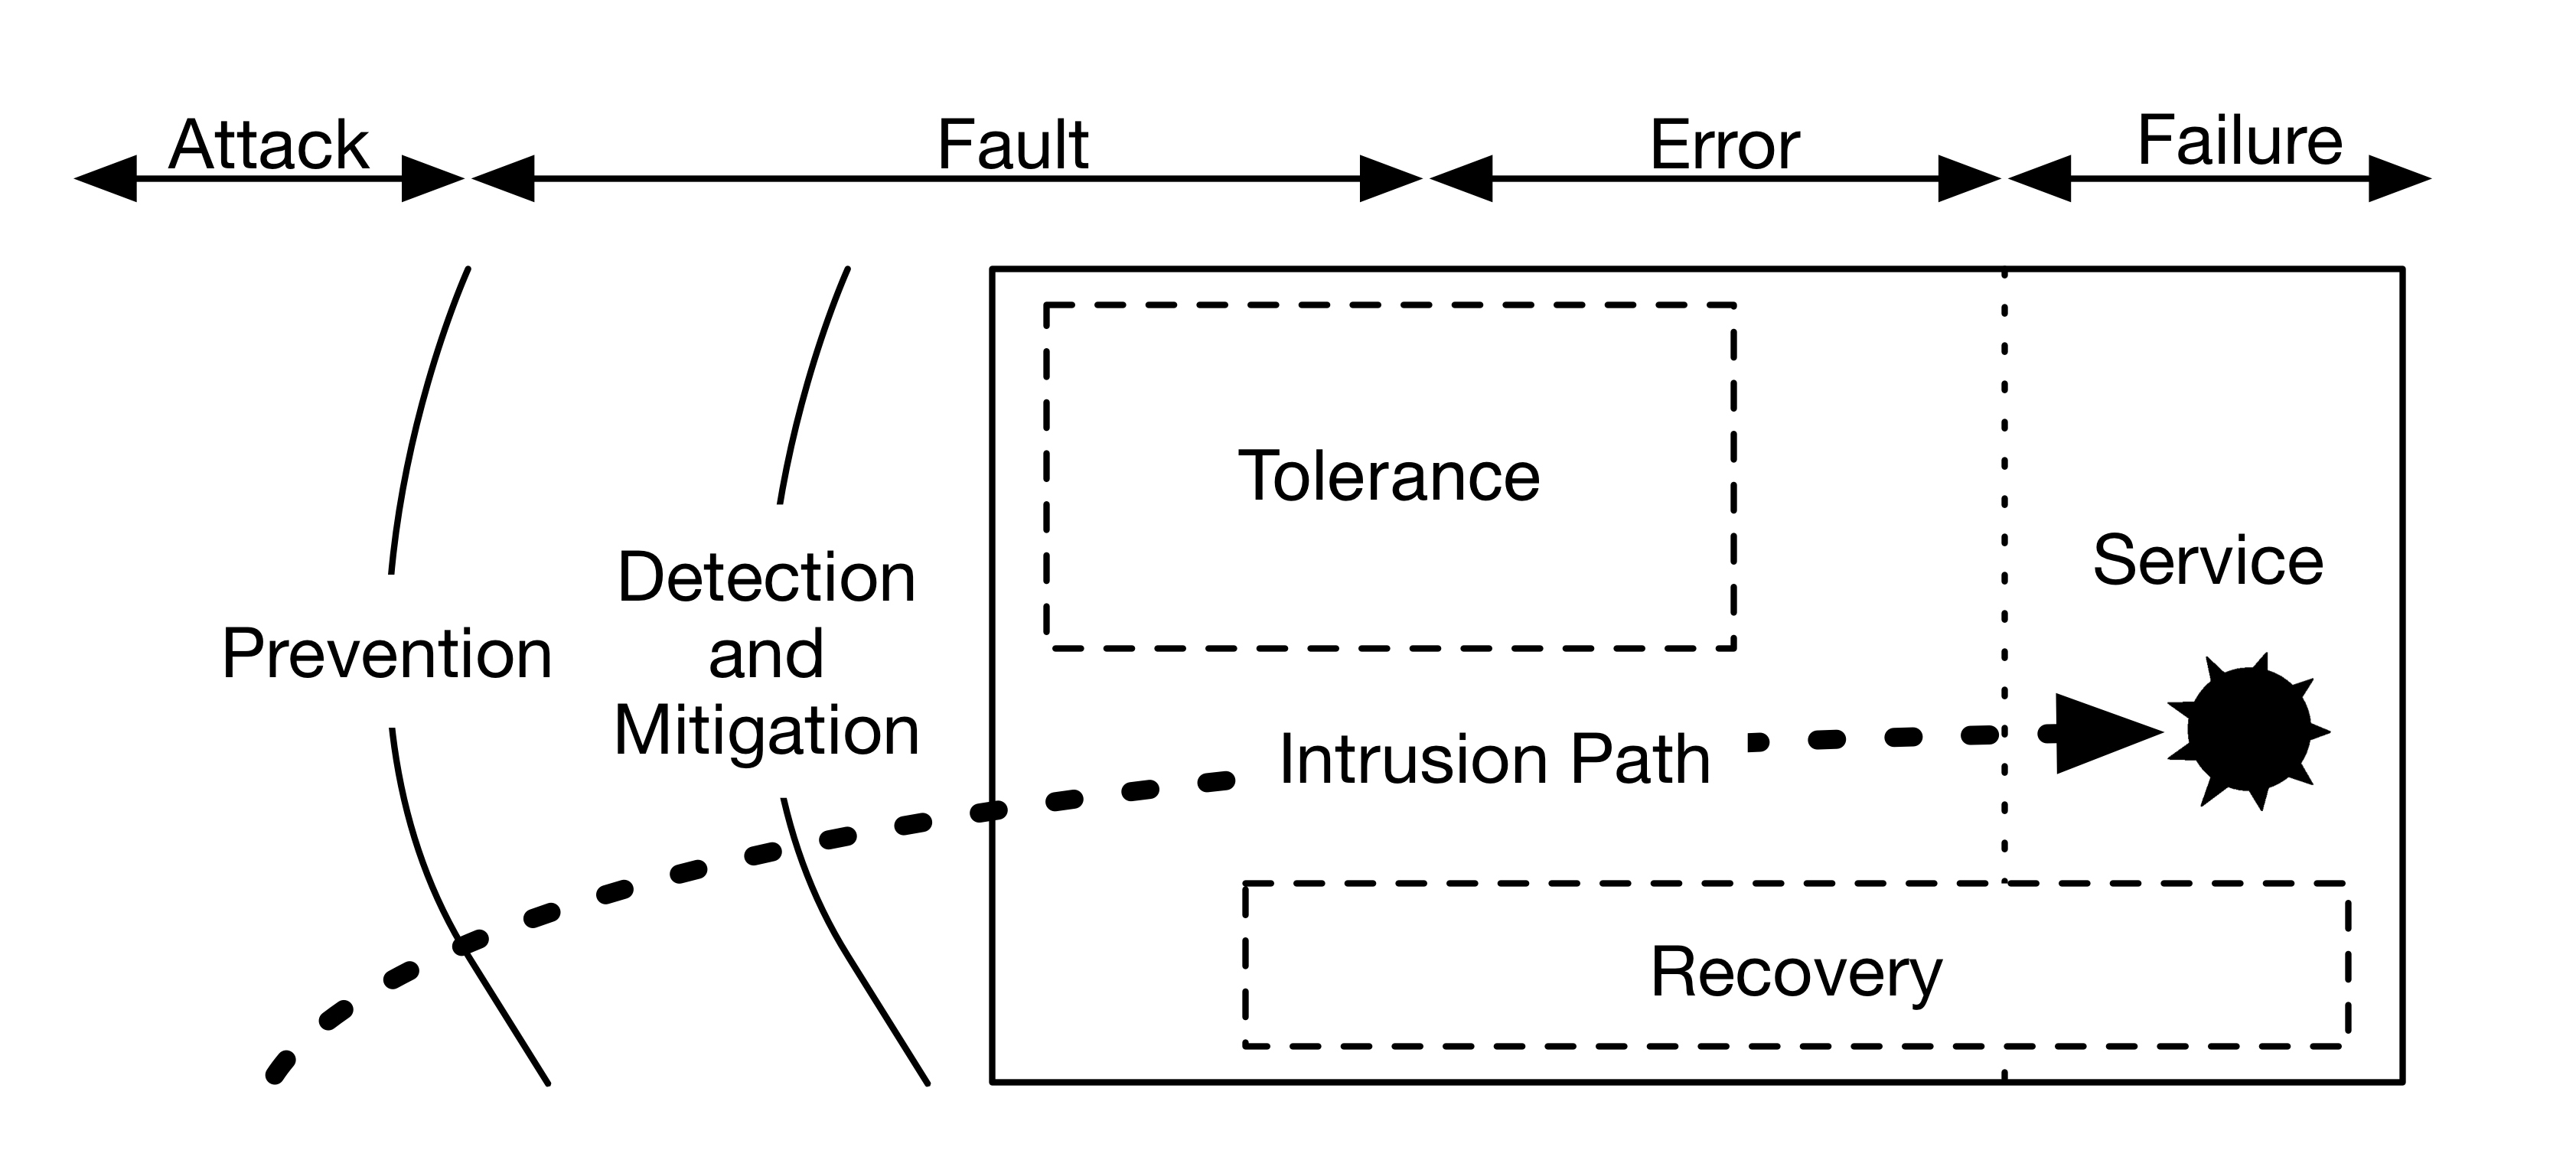
\includegraphics[width=110mm]{images/intrusion}
  \caption{Intrusion path across the system}
  \label{fig:intrusion_path}
\end{figure}

%prevention
\emph{Intrusion forecast and prevention} are realized by design and they seek to prevent future attackers from exploiting vulnerabilities. However, preventing intrusions by design is hard. Software has flaws due to its complexity and budget/time constraints \cite{Charette2005,Landwehr1992}. System administrators, as humans, can make security configuration mistakes or users may grant access to attackers \cite{Brown2001}. Moreover attackers can spend years developing new ingenious and unanticipated intrusions having access to what protects the system while the guardians have to predict them. Due to this asymmetry, it is arguably impossible to protect all vulnerabilities by design. Therefore the vulnerabilities of prevention mechanisms can be exploited successfully leading to an intrusion. A vast number of vulnerabilities and attacks are listed for instance in the National Vulnerability Database \cite{nistNVD}.\\

\emph{Intrusion detection and mitigation} mechanisms monitor the system to detect suspicious actions that may be connected with an intrusion. However, intrusion detection systems turn the system attack-aware but not attack-resilient, that is, they cannot maintain the integrity and availability of the system in face of attacks \cite{Ammann2002}. Intrusion detection systems may not detect unknown vulnerabilities. More, attackers may use encrypted actions or use legitimate requests.\\

%Intrusion Tolerance
\emph{Intrusion tolerance} is the last line of defense against attacks before the system failure occurs (Fig. \ref{fig:intrusion_path}). Intrusion tolerance is the ability of a system to keep providing a, possibly degraded but adequate, service during and after an intrusion \cite{Stavridou2001a}. Instead of trying to prevent every single intrusion, these are allowed, but tolerated. The system has mechanisms to prevent the intrusion from generating a system failure \cite{Verissimo2003}. Intrusion tolerance mechanisms hide the errors effects using redundancy mechanisms or using intrusion recovery systems, which detect, process and recover from intrusions.\\

Many intrusion tolerance mechanisms are based on replicating state with Byzantine fault-tolerant protocols \cite{Schneider1990,Castro2002,Veronese2011}. The idea is to ensure that a service remains operational and correct as long as no more than a certain number of replicas are compromised. Replicas can be implemented in different manners to provide diversity, to reduce the risk of common failure modes. In addition, a proactive recovery mechanism can reboot the replicas periodically to rejuvenate and restore their soft-state and security assets, e.g., keys \cite{Candea2001,Castro2002,Sousa2010}. In \emph{disaster recovery} solutions, the state is replicated in remote sites, allowing the recovery from catastrophes that destroy a site \cite{Wood2010}.\\

The above-mentioned replication mechanisms for intrusion tolerance can tolerate some intrusions targeted at design faults (vulnerabilities), as long as diversity is used. However, most of the fault tolerance mechanisms do not prevent accidentally or malicious faults at application level, e.g., using valid user requests. Most of state replication mechanisms facilitate the damage to spread from one site to many sites as they copy data without distinguishing between legitimate and malicious sources. Furthermore, most of proactive recovery techniques rejuvenate only the application soft-state but intrusions can affect its persistent state. Consequently, intrusions may transverse these intrusion tolerance mechanisms and cause a system failure. 

